\section{Statická kondenzace}

Při výpočtu prutových konstrukcí se lze často setkat s kloubovým připojení prutů. V případě na obr. \ref{fig:node_phis} se vy styčníku stýkají 4 pruty, posunutí \gls{u_i}[a] a \gls{w_i}[a] jsou jednoznačně popsány, ale pootočení koncových průřezů levého a pravého prutu jsou různá od pootočení \gls{phi_i}[a]. Ve styčníku tedy vzniká celkem 5 neznámých, 2 posunutí a 3 pootočení. Podmínky rovnováhy pro pootočení kloubově připojených prutů požadují, aby ohybový moment ve styčníku byl roven nule. Podmínku nulového koncového momentu lze uplatnit přímo v matici tuhosti prutového prvku a do globálních podmínek rovnováhy přičíst síly z prutu, který je typu vetknutí-kloub.

\begin{figure}[H]
    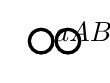
\begin{tikzpicture}
    \scaling{2};

    \point{a}{0}{-1};
    \point{b}{1}{0};
    \point{c}{0}{1};
    \point{d}{-1}{0};
    \point{e}{0}{0};

    \beam{1}{a}{e}[1][1];
    \beam{1}{d}{e}[1][1];
    \beam{1}{e}{b}[1][1];
    \beam{1}{e}{c}[1][1];

    \draw[fill=white, very thick] (-0.17,0) circle (.15);
    \draw[fill=white, very thick] (0.17, 0) circle (.15);

    \notation{1}{e}{$a$}[above right=.12 and .12];
    \notation{4}{d}{e}[$\text{A}$][.2];
    \notation{4}{b}{e}[$\text{B}$][.2];
    \notation{4}{a}{e}[$\text{C}$][.2];
    \notation{4}{e}{c}[$\text{D}$][.8];
\end{tikzpicture}
    \caption{Styčník s kloubově připojenými pruty}
    \label{fig:node_phis}
\end{figure}

Matici tuhosti prvku, vektor uzlových posunutí a vektor zatížení rozdělíme na submatice odpovídající ponechaným (index $a$) a kondenzovaným (index $b$) stupňům volnosti,
\begin{equation}
    \begin{bmatrix}
        \gls{K}_{aa} & \gls{K}_{ab} \\
        \gls{K}_{ba} & \gls{K}_{bb}
    \end{bmatrix}
    \begin{Bmatrix}
        \gls{d}_a \\
        \gls{d}_b
    \end{Bmatrix}
    =
    \begin{Bmatrix}
        \matr{f}_a \\
        \matr{f}_b
    \end{Bmatrix}.
\end{equation}

Z druhé rovnice vyjádříme $\gls{d}_{b}$,
\begin{equation}
    \begin{aligned}
        \gls{K}_{ba} \gls{d}_a + \gls{K}_{bb} \gls{d}_{b} = \matr{f}_b \\
        \gls{d}_{b} = \gls{K}_{bb}^{-1} \left( \matr{f}_{b} - \gls{K}_{ba} \gls{d}_a \right).
    \end{aligned}
\end{equation}

Po dosazení do první rovnice obdržíme
\begin{equation} \label{eq:condensation}
    \begin{aligned}
        \gls{K}_{aa} \gls{d}_a + \gls{K}_{ab} \left(\gls{K}_{bb}^{-1} \left( \matr{f}_{b} - \gls{K}_{ba} \gls{d}_a \right)\right) &= \matr{f}_a \\
        \left(\gls{K}_{aa} - \gls{K}_{ab} \gls{K}_{bb}^{-1} \gls{K}_{ba}\right) \gls{d}_a &= \matr{f}_a - \gls{K}_{ab} \gls{K}_{bb}^{-1} \matr{f}_{b}\\
        \gls{K}^* \gls{d}_{a} &= \matr{f}^*.
    \end{aligned}
\end{equation}
 
Uvedeme příklad kondenzace matice tuhosti pro prut typu vetknutí-kloub z matice tuhosti odvozené v kap. \ref{sec:K_eb_beam}.

\begin{figure}[H]
    \begin{tikzpicture}[>={Stealth[inset=0pt,length=8pt,angle'=28,round]}]
    \point{a}{0}{0};
    \point{b}{8}{0};

    \beam{1}{a}{b};

    \notation{2}{a}{$a$};
    \notation{1}{b}{$b$};
    
    \draw[->] (0, 0) -- (0, 1.5) node[text=ctublue,above] {$w_a$};
    \draw[->,domain=300:30] plot ({cos(\x)}, {sin(\x)}) node[text=ctublue, above right] {$\varphi_a$};
    \draw[->] (8, 0) -- (8, 1.5) node[text=ctublue,above] {$w_b$};
    \draw[->,domain=300:30] plot ({8+cos(\x)}, {sin(\x)}) node[text=ctublue, above right] {$\varphi_b, M_b=0$};
    \draw[fill=white, very thick] (8, 0) circle (.15);
\end{tikzpicture}
    \caption{Prut typu vetknutí-kloub}
    \label{fig:beam_clamped}
\end{figure}


Importujeme knihovnu SymPy.
\begin{tcolorbox}[breakable, size=fbox, boxrule=1pt, pad at break*=1mm,colback=cellbackground, colframe=cellborder]
    \prompt{In}{incolor}{1}{\boxspacing}
    \begin{Verbatim}[commandchars=\\\{\}]
    \PY{k+kn}{import} \PY{n+nn}{sympy} \PY{k}{as} \PY{n+nn}{smp}
    \end{Verbatim}
\end{tcolorbox}
    
Definujeme proměnné.
\begin{tcolorbox}[breakable, size=fbox, boxrule=1pt, pad at break*=1mm,colback=cellbackground, colframe=cellborder]
    \prompt{In}{incolor}{2}{\boxspacing}
    \begin{Verbatim}[commandchars=\\\{\}]
    \PY{n}{E}\PY{p}{,} \PY{n}{I}\PY{p}{,} \PY{n}{L} \PY{o}{=} \PY{n}{smp}\PY{o}{.}\PY{n}{symbols}\PY{p}{(}\PY{l+s+s1}{\PYZsq{}}\PY{l+s+s1}{E I L}\PY{l+s+s1}{\PYZsq{}}\PY{p}{)}
    \PY{n}{w\PYZus{}a}\PY{p}{,} \PY{n}{phi\PYZus{}a}\PY{p}{,} \PY{n}{w\PYZus{}b}\PY{p}{,} \PY{n}{phi\PYZus{}b} \PY{o}{=} \PY{n}{smp}\PY{o}{.}\PY{n}{symbols}\PY{p}{(}
        \PY{l+s+s1}{\PYZsq{}}\PY{l+s+s1}{w\PYZus{}a varphi\PYZus{}a w\PYZus{}b varphi\PYZus{}b}\PY{l+s+s1}{\PYZsq{}}
    \PY{p}{)}
    \end{Verbatim}
\end{tcolorbox}

Definujeme matici tuhosti \gls{K}.
\begin{tcolorbox}[breakable, size=fbox, boxrule=1pt, pad at break*=1mm,colback=cellbackground, colframe=cellborder]
    \prompt{In}{incolor}{3}{\boxspacing}
    \begin{Verbatim}[commandchars=\\\{\}]
    \PY{n}{K} \PY{o}{=} \PY{n}{E} \PY{o}{*} \PY{n}{I} \PY{o}{/} \PY{n}{L} \PY{o}{*} \PY{n}{smp}\PY{o}{.}\PY{n}{Matrix}\PY{p}{(}
        \PY{p}{[}
            \PY{p}{[}\PY{l+m+mi}{12}\PY{o}{/}\PY{n}{L}\PY{o}{*}\PY{o}{*}\PY{l+m+mi}{2}\PY{p}{,} \PY{o}{\PYZhy{}}\PY{l+m+mi}{6}\PY{o}{/}\PY{n}{L}\PY{p}{,} \PY{o}{\PYZhy{}}\PY{l+m+mi}{12}\PY{o}{/}\PY{n}{L}\PY{o}{*}\PY{o}{*}\PY{l+m+mi}{2}\PY{p}{,} \PY{o}{\PYZhy{}}\PY{l+m+mi}{6}\PY{o}{/}\PY{n}{L}\PY{p}{]}\PY{p}{,}
            \PY{p}{[}\PY{o}{\PYZhy{}}\PY{l+m+mi}{6}\PY{o}{/}\PY{n}{L}\PY{p}{,} \PY{l+m+mi}{4}\PY{p}{,} \PY{l+m+mi}{6}\PY{o}{/}\PY{n}{L}\PY{p}{,} \PY{l+m+mi}{2}\PY{p}{]}\PY{p}{,}
            \PY{p}{[}\PY{o}{\PYZhy{}}\PY{l+m+mi}{12}\PY{o}{/}\PY{n}{L}\PY{o}{*}\PY{o}{*}\PY{l+m+mi}{2}\PY{p}{,} \PY{l+m+mi}{6}\PY{o}{/}\PY{n}{L}\PY{p}{,} \PY{l+m+mi}{12}\PY{o}{/}\PY{n}{L}\PY{o}{*}\PY{o}{*}\PY{l+m+mi}{2}\PY{p}{,} \PY{l+m+mi}{6}\PY{o}{/}\PY{n}{L}\PY{p}{]}\PY{p}{,}
            \PY{p}{[}\PY{o}{\PYZhy{}}\PY{l+m+mi}{6}\PY{o}{/}\PY{n}{L}\PY{p}{,} \PY{l+m+mi}{2}\PY{p}{,} \PY{l+m+mi}{6}\PY{o}{/}\PY{n}{L}\PY{p}{,} \PY{l+m+mi}{4}\PY{p}{]}
        \PY{p}{]}
    \PY{p}{)}
    
    \PY{n}{K}
    \end{Verbatim}
\end{tcolorbox}
     
                
\prompt{Out}{outcolor}{3}{}
    
    $\displaystyle \left[\begin{matrix}\frac{12 E I}{L^{3}} & - \frac{6 E I}{L^{2}} & - \frac{12 E I}{L^{3}} & - \frac{6 E I}{L^{2}}\\- \frac{6 E I}{L^{2}} & \frac{4 E I}{L} & \frac{6 E I}{L^{2}} & \frac{2 E I}{L}\\- \frac{12 E I}{L^{3}} & \frac{6 E I}{L^{2}} & \frac{12 E I}{L^{3}} & \frac{6 E I}{L^{2}}\\- \frac{6 E I}{L^{2}} & \frac{2 E I}{L} & \frac{6 E I}{L^{2}} & \frac{4 E I}{L}\end{matrix}\right]$
    
        
\vspace{0.3cm}
Matici \gls{K} rozdělíme na submatice.   
\begin{tcolorbox}[breakable, size=fbox, boxrule=1pt, pad at break*=1mm,colback=cellbackground, colframe=cellborder]
    \prompt{In}{incolor}{4}{\boxspacing}
    \begin{Verbatim}[commandchars=\\\{\}]
    \PY{n}{K\PYZus{}aa} \PY{o}{=} \PY{n}{K}\PY{p}{[}\PY{l+m+mi}{0}\PY{p}{:}\PY{l+m+mi}{3}\PY{p}{,} \PY{l+m+mi}{0}\PY{p}{:}\PY{l+m+mi}{3}\PY{p}{]}
    \PY{n}{K\PYZus{}aa}
    \end{Verbatim}
\end{tcolorbox}
     
                
\prompt{Out}{outcolor}{4}{}
    
    $\displaystyle \left[\begin{matrix}\frac{12 E I}{L^{3}} & - \frac{6 E I}{L^{2}} & - \frac{12 E I}{L^{3}}\\- \frac{6 E I}{L^{2}} & \frac{4 E I}{L} & \frac{6 E I}{L^{2}}\\- \frac{12 E I}{L^{3}} & \frac{6 E I}{L^{2}} & \frac{12 E I}{L^{3}}\end{matrix}\right]$
    
        
    
\begin{tcolorbox}[breakable, size=fbox, boxrule=1pt, pad at break*=1mm,colback=cellbackground, colframe=cellborder]
    \prompt{In}{incolor}{5}{\boxspacing}
    \begin{Verbatim}[commandchars=\\\{\}]
    \PY{n}{K\PYZus{}ab} \PY{o}{=} \PY{n}{K}\PY{p}{[}\PY{l+m+mi}{0}\PY{p}{:}\PY{l+m+mi}{3}\PY{p}{,} \PY{l+m+mi}{3}\PY{p}{:}\PY{p}{]}
    \PY{n}{K\PYZus{}ab}
    \end{Verbatim}
\end{tcolorbox}
     
                
\prompt{Out}{outcolor}{5}{}
    
    $\displaystyle \left[\begin{matrix}- \frac{6 E I}{L^{2}}\\\frac{2 E I}{L}\\\frac{6 E I}{L^{2}}\end{matrix}\right]$

        
    
\begin{tcolorbox}[breakable, size=fbox, boxrule=1pt, pad at break*=1mm,colback=cellbackground, colframe=cellborder]
    \prompt{In}{incolor}{6}{\boxspacing}
    \begin{Verbatim}[commandchars=\\\{\}]
    \PY{n}{K\PYZus{}ba} \PY{o}{=} \PY{n}{K}\PY{p}{[}\PY{l+m+mi}{3}\PY{p}{:}\PY{p}{,} \PY{l+m+mi}{0}\PY{p}{:}\PY{l+m+mi}{3}\PY{p}{]}
    \PY{n}{K\PYZus{}ba}
    \end{Verbatim}
\end{tcolorbox}
     
                
\prompt{Out}{outcolor}{6}{}
    
    $\displaystyle \left[\begin{matrix}- \frac{6 E I}{L^{2}} & \frac{2 E I}{L} & \frac{6 E I}{L^{2}}\end{matrix}\right]$
    
        
    
\begin{tcolorbox}[breakable, size=fbox, boxrule=1pt, pad at break*=1mm,colback=cellbackground, colframe=cellborder]
    \prompt{In}{incolor}{7}{\boxspacing}
    \begin{Verbatim}[commandchars=\\\{\}]
    \PY{n}{K\PYZus{}bb} \PY{o}{=} \PY{n}{K}\PY{p}{[}\PY{l+m+mi}{3}\PY{p}{:}\PY{p}{,} \PY{l+m+mi}{3}\PY{p}{:}\PY{p}{]}
    \PY{n}{K\PYZus{}bb}
    \end{Verbatim}
\end{tcolorbox}
     
                
\prompt{Out}{outcolor}{7}{}
    
    $\displaystyle \left[\begin{matrix}\frac{4 E I}{L}\end{matrix}\right]$

\vspace{0.3cm}
Provedeme statickou kondenzaci podle vztahu \ref{eq:condensation}.    
\begin{tcolorbox}[breakable, size=fbox, boxrule=1pt, pad at break*=1mm,colback=cellbackground, colframe=cellborder]
    \prompt{In}{incolor}{8}{\boxspacing}
    \begin{Verbatim}[commandchars=\\\{\}]
    \PY{n}{K\PYZus{}condensed} \PY{o}{=} \PY{n}{K\PYZus{}aa} \PY{o}{\PYZhy{}} \PY{n}{K\PYZus{}ab} \PY{o}{@} \PY{n}{K\PYZus{}bb}\PY{o}{.}\PY{n}{inv}\PY{p}{(}\PY{p}{)} \PY{o}{@} \PY{n}{K\PYZus{}ba}
    \PY{n}{K\PYZus{}condensed}
    \end{Verbatim}
\end{tcolorbox}
     
                
\prompt{Out}{outcolor}{8}{}
    
    $\displaystyle \left[\begin{matrix}\frac{3 E I}{L^{3}} & - \frac{3 E I}{L^{2}} & - \frac{3 E I}{L^{3}}\\- \frac{3 E I}{L^{2}} & \frac{3 E I}{L} & \frac{3 E I}{L^{2}}\\- \frac{3 E I}{L^{3}} & \frac{3 E I}{L^{2}} & \frac{3 E I}{L^{3}}\end{matrix}\right]$